\chapter{Spin, Messung und der zweidimensionale Zustandsraum}

\lectureoverview{Ein Spin ist gerichtet, doch jede Messung einer seiner Komponenten liefert nur \(+1\) oder \(-1\). Zunächst formulieren wir dieses operationelle Rätsel und sehen dann, warum die gewöhnliche Mengenlogik bei inkompatiblen Messungen versagt. Der passende mathematische Rahmen ist ein zweidimensionaler komplexer Vektorraum: Wahrscheinlichkeiten ergeben sich aus Amplituden, unterscheidbare Alternativen sind orthogonal, und die Basen up--down, right--left und in--out codieren drei räumliche Richtungen, ohne einen Zustandsvektor in einen gewöhnlichen Pfeil zu verwandeln.}

\section{Vom Qubit zum Spin}

Das zuvor als Qubit eingeführte Zweizustandssystem nennen wir nun \emph{Spin}. Mit dieser Namensänderung kommt die räumliche Richtung ins Spiel; zugleich entsteht jedoch eine Gefahr durch das Wort \emph{Vektor}. Zwei verschiedene Objekte müssen auseinandergehalten werden:

\begin{definition}
Ein \emph{Dreiervektor} ist ein gewöhnlicher reeller Vektor im dreidimensionalen Raum. Mit \emph{Vektor} ohne nähere Bestimmung ist ein Element eines abstrakten Vektorraums gemeint, etwa des komplexen Zustandsraums der Quantenmechanik.
\end{definition}

Ein Spin kann relativ zu einer Achse im gewöhnlichen Raum präpariert werden. Sein Zustand wird jedoch durch einen abstrakten Vektor dargestellt. Die Beziehung zwischen diesen beiden Aussagen gehört zu dem, was wir erst noch herausfinden müssen; aus einer Abbildung lässt sie sich nicht einfach ableiten.

\section{Warum sich der Messapparat nicht entfernen lässt}

Die klassische Mechanik verleitet uns zu der Vorstellung eines idealen Beobachters, der etwas über ein System erfahren kann, ohne es stärker als gewünscht zu stören. Nehmen wir etwa an, wir wollten einen makroskopischen Gegenstand sehen. Wir beleuchten ihn, sammeln das reflektierte Licht mit einer Linse und verstärken das Bild. Das Licht übt zwar eine Kraft aus, doch in der klassischen Idealisierung kann seine Intensität verringert und zugleich die Verstärkung erhöht werden. Die Störung lässt sich beliebig klein machen, ohne die Vorstellung einer Messung aufzugeben.

In der Quantenmechanik funktioniert dieses Grenzverfahren nicht. Ein Messapparat lässt sich verbessern, abschirmen und kalibrieren, doch eine Messung kann im Allgemeinen nicht zugleich informativ und beliebig störungsfrei sein. Am System ändert sich etwas. Das bedeutet weder, dass jede Messung jede Eigenschaft zerstört, noch, dass sich das Ergebnis nicht reproduzieren lässt. Es bedeutet, dass der Messapparat Teil der physikalischen Fragestellung ist und der Zustand nach der Messung nicht außer Acht gelassen werden kann.

Für den Moment betrachten wir den Messapparat als Blackbox mit zwei Eigenschaften: Er lässt sich räumlich ausrichten, und seine Anzeige hält entweder \(+1\) oder \(-1\) fest. Ein kleiner Pfeil an der Tafel ist eine praktische Kennzeichnung für einen präparierten Spin:

\begin{figure}[htbp]
\centering
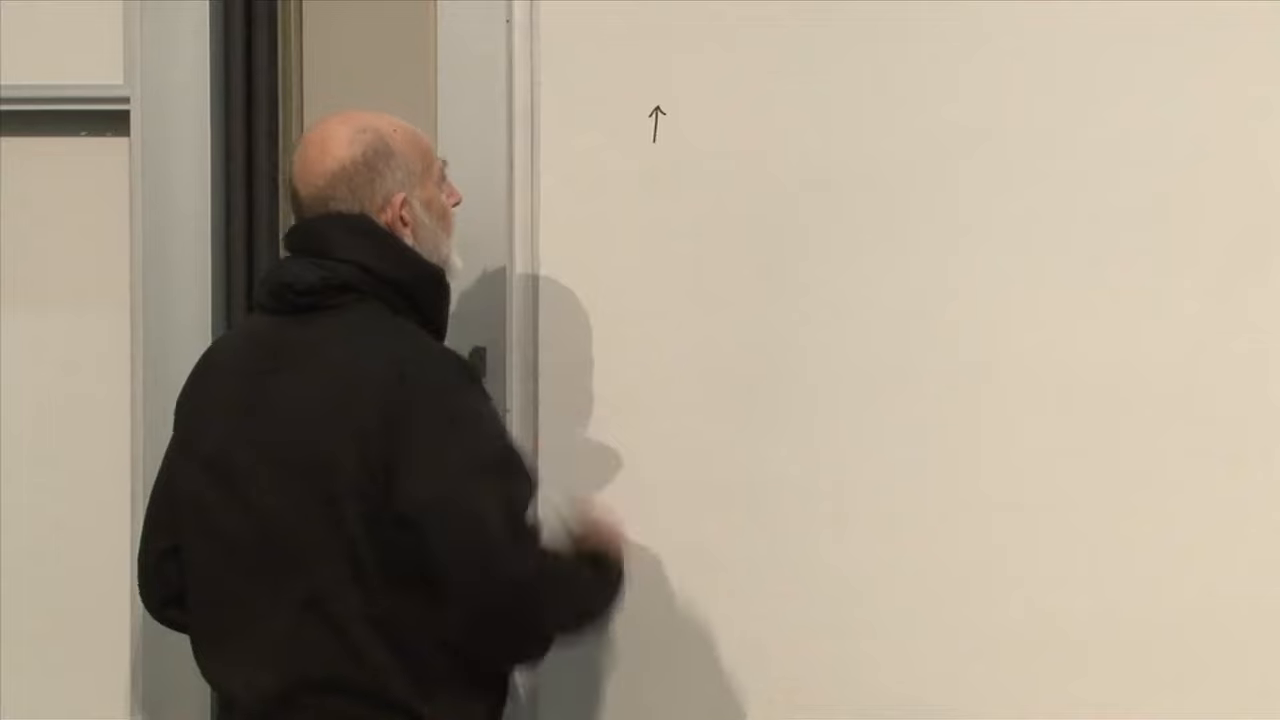
\includegraphics[width=0.64\textwidth]{lecture_02_figure_02.png}
\caption{Die erste vorläufige Markierung für einen entlang einer Achse präparierten Spin. Der Pfeil kennzeichnet eine Präparation; er ist noch kein klassisches Modell des Zustands.}
\lectureframe{00:05:15}
\end{figure}

Wählen wir die Achsen so, dass \(z\) an der Tafel nach oben, \(x\) nach rechts und \(y\) aus der Tafel heraus zeigt. Ist der Messapparat entlang einer Einheitsrichtung \(\hat m\) ausgerichtet, lautet sein Ergebnis
\begin{equation}
\sigma_{\hat m}=\pm1.
\end{equation}
Insbesondere gilt
\[
\sigma_z=\pm1,\qquad \sigma_x=\pm1,\qquad \sigma_y=\pm1.
\]
Das Wort \emph{Komponente} ist hier zunächst operationell zu verstehen: \(\sigma_z\) ist das, was der ausgerichtete Messapparat anzeigt, wenn er entlang \(z\) weist. Es ist noch nicht die \(z\)-Komponente eines verborgenen klassischen Pfeils.

\subsection{Wiederholbarkeit und Störung}

Angenommen, eine \(z\)-Messung ergibt \(+1\). Ohne zwischenzeitliche Operation liefert auch eine zweite \(z\)-Messung wieder \(+1\), ebenso alle weiteren Wiederholungen. Die erste Messung hat einen Zustand präpariert, in dem dieselbe Frage eine eindeutige Antwort hat.

\begin{classroomqa}
\audiencequestion{Wenn eine Quantenmessung den Spin stört, warum liefert eine unmittelbar anschließende Wiederholung dann dasselbe Ergebnis?}
\lecturerresponse{Die Störung erfolgt nicht wahllos. Eine Messung von \(\sigma_z\) kann das Ergebnis einer späteren \(x\)- oder \(y\)-Messung verändern und zugleich dafür sorgen, dass der neu gemessene Wert von \(\sigma_z\) reproduzierbar bleibt. Ein brauchbares Experiment setzt genau diese begrenzte Form von Stabilität voraus.}
\end{classroomqa}

Drehen wir den Messapparat nun um \(180^\circ\). Ein Spin, der bei Ausrichtung nach oben \(+1\) ergab, liefert bei umgekehrter Ausrichtung \(-1\). Richten wir den Apparat wieder aufrecht aus, ist das Ergebnis \(+1\). Die Orientierung spielt also eine Rolle. Ein Thermometer würde nicht eine negative Temperatur anzeigen, nur weil man es auf den Kopf stellt; der Spinanalysator verhält sich anders, weil er eine gerichtete Frage stellt.

\begin{figure}[htbp]
\centering
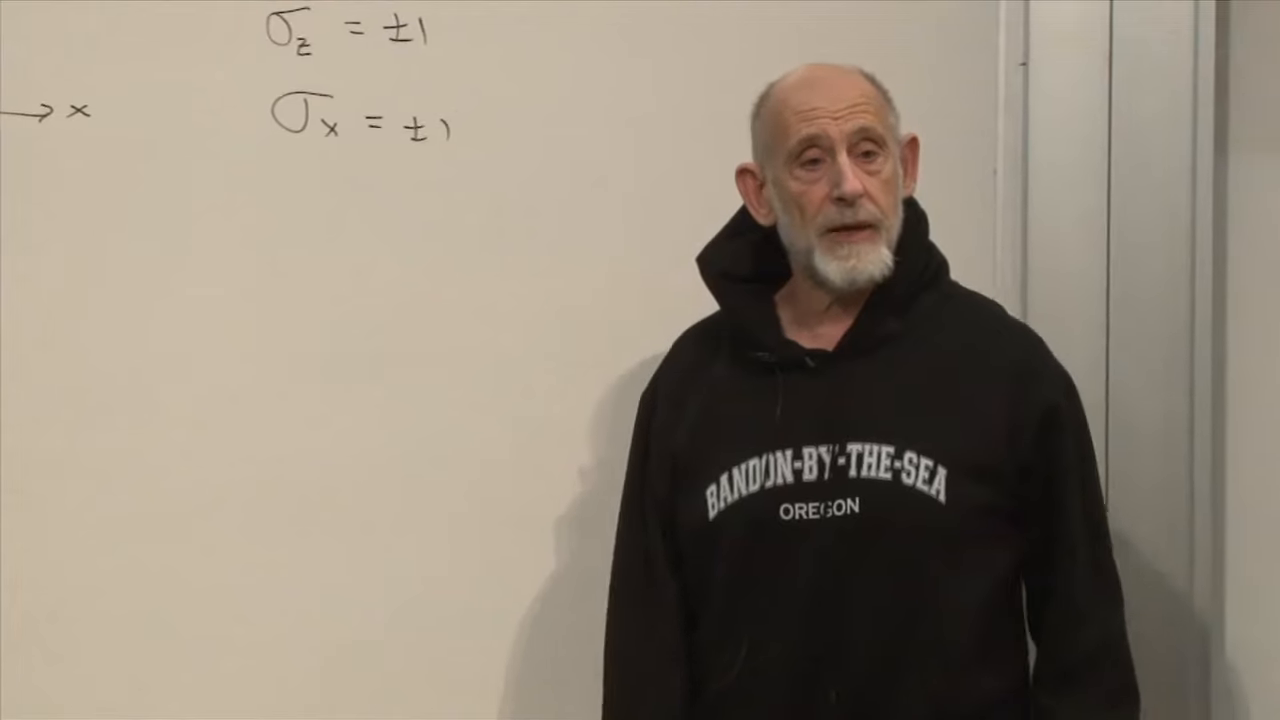
\includegraphics[width=0.72\textwidth]{lecture_02_figure_03.png}
\caption{Die Tafel hält die zweifachen Kennzeichnungen \(\sigma_z=\pm1\) und \(\sigma_x=\pm1\) sowie den Hinweis auf die \(x\)-Achse fest.}
\lectureframe{00:12:46}
\end{figure}

Der Unterschied zu einem klassischen Einheitsvektor ist unmittelbar klar. Klassische Komponenten können kontinuierlich zwischen \(-1\) und \(+1\) liegen. Ein Einheitsvektor senkrecht zur \(x\)-Achse hat eine \(x\)-Komponente von null. Ein Spinanalysator, der entlang \(x\) ausgerichtet ist, zeigt dagegen niemals null an. Er zeigt \(+1\) oder \(-1\), selbst wenn der Spin entlang \(z\) präpariert wurde.

\section{Einzelergebnisse und vektorartige Mittelwerte}

Wir präparieren einen Spin, indem wir \(\sigma_z=+1\) erhalten, und messen anschließend \(\sigma_x\). Bei der Hälfte identisch präparierter Versuche ergibt sich \(+1\), bei der anderen Hälfte \(-1\). Somit gilt
\begin{equation}
\langle \sigma_x\rangle=0.
\end{equation}
Dieselbe Präparation ergibt
\begin{equation}
\langle \sigma_y\rangle=0.
\end{equation}
Umgekehrt hat ein mit \(\sigma_x=+1\) präparierter Spin bei einer anschließenden \(z\)- oder \(y\)-Messung für beide Ergebnisse die gleiche Wahrscheinlichkeit.

In dieser Aussage stecken zwei verschiedene Experimente. Wiederholte Messungen von \(\sigma_x\) am \emph{selben} Spin nach dem ersten \(x\)-Ergebnis bestätigen lediglich dieses Ergebnis. Um die Fünfzig--fünfzig-Statistik zu erhalten, benötigt man viele Spins, die im selben \(z\)-Zustand präpariert wurden, oder einen Spin, der vor jeder \(x\)-Messung wiederholt in denselben Präparationszustand zurückversetzt wird.

\begin{classroomqa}
\audiencequestion{Was geschieht, wenn ein Spin nicht gezielt präpariert wurde, bevor er in den Messapparat gelangt?}
\lecturerresponse{Das Ergebnis ist weiterhin \(+1\) oder \(-1\), doch die Wahrscheinlichkeiten hängen vom tatsächlichen Zustand des Spins ab. Eine Präparation ist das kontrollierte Verfahren, das wiederholte Versuche vergleichbar macht. Findet zwischen zwei Messungen eine unbekannte Manipulation statt, ist die Wiederholbarkeit nicht mehr garantiert; geschieht nichts, lässt sich das Ergebnis für dieselbe Komponente reproduzieren.}
\end{classroomqa}

\subsection{Zwei beliebige Richtungen}

Wir präparieren den Spin entlang einer Einheitsrichtung \(\hat n\), indem ein entlang \(\hat n\) ausgerichteter Analysator \(+1\) ergibt. Anschließend messen wir entlang einer anderen Einheitsrichtung \(\hat m\). Jeder Versuch liefert weiterhin nur \(\pm1\), doch der Mittelwert über identisch präparierte Versuche ist
\begin{equation}
\boxed{\langle\sigma_{\hat m}\rangle=\hat n\cdot\hat m
=\cos\theta_{nm}.}
\label{eq:spin-average}
\end{equation}
An der Tafel verwenden wir die kürzere Schreibweise \(\langle\sigma_m\rangle=n\cdot m\):

\begin{figure}[htbp]
\centering
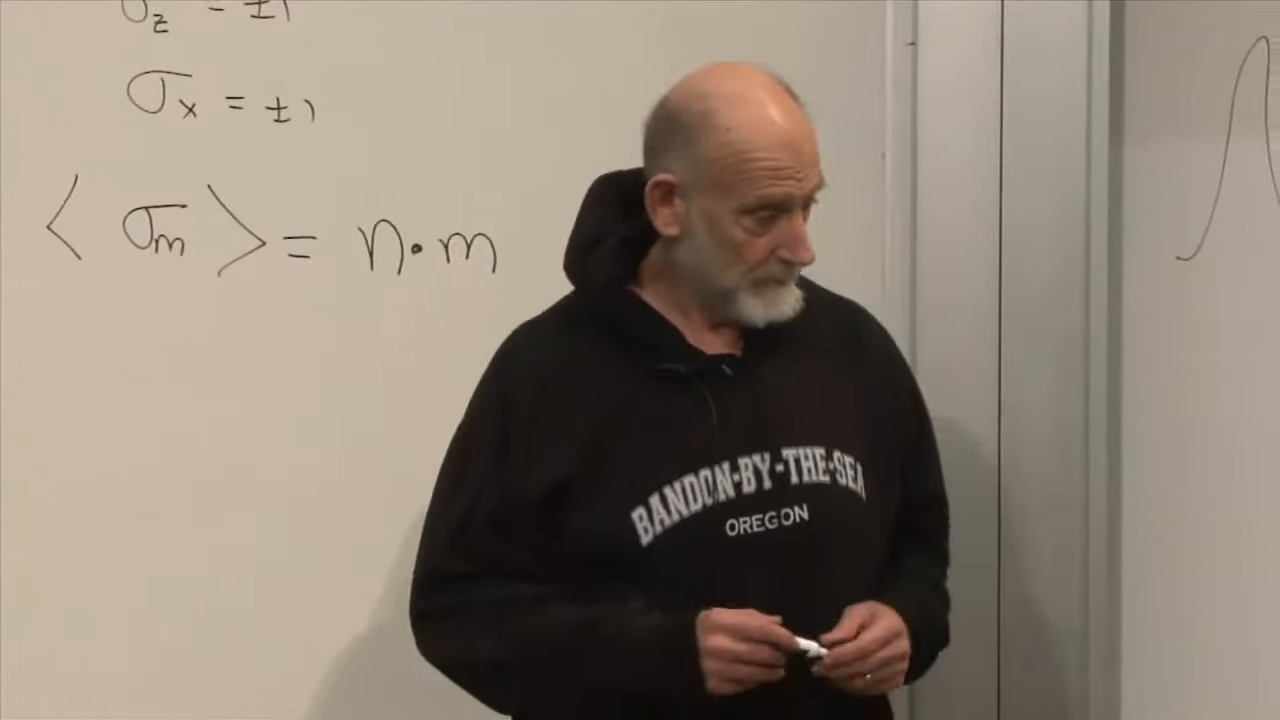
\includegraphics[width=0.74\textwidth]{lecture_02_figure_04.png}
\caption{Das vektorartige Gesetz gilt für den Mittelwert über ein Ensemble, nicht für ein einzelnes Ergebnis \(\pm1\).}
\lectureframe{00:23:22}
\end{figure}

Gleichung~\eqref{eq:spin-average} umfasst auch die früheren Fälle. Für \(\hat m=\hat n\) ist der Mittelwert \(+1\); da kein Ergebnis größer als \(+1\) sein kann, ergibt jeder Versuch \(+1\). Für \(\hat m=-\hat n\) ergibt jeder Versuch \(-1\). Senkrechte Achsen ergeben einen Mittelwert von null und gleiche Häufigkeiten.

Bezeichnen \(p_+\) und \(p_-\) die Wahrscheinlichkeiten der beiden möglichen Ergebnisse, so gilt
\[
p_++p_-=1,\qquad p_+-p_-=\hat n\cdot\hat m.
\]
Folglich
\begin{equation}
p_\pm=\frac{1\pm\hat n\cdot\hat m}{2}.
\label{eq:direction-probabilities}
\end{equation}
\editorialnote{In der Vorlesung werden die beiden Ergebnisse und ihr Mittelwert angegeben. Gleichung~\eqref{eq:direction-probabilities} folgt algebraisch unmittelbar aus diesen beiden Angaben.}

\begin{classroomqa}
\audiencequestion{Ist die Größe in den spitzen Klammern ein \emph{Erwartungswert} oder ein gewöhnlicher Mittelwert?}
\lecturerresponse{Sie ist der Mittelwert der aufgezeichneten Ergebnisse aus vielen Wiederholungen. \emph{Erwartungswert} ist die übliche Bezeichnung; eine zusätzliche Art der Mittelung ist hier aber nicht gemeint. Der Messapparat liefert eine Liste aus \(+1\) und \(-1\); die Klammern bezeichnen im Grenzfall eines großen Ensembles das arithmetische Mittel dieser Liste.}
\end{classroomqa}

\begin{classroomqa}
\audiencequestion{Hatte der Pfeil \(\hat n\) schon eine geometrische Bedeutung, bevor das Gesetz für den Mittelwert bekannt war?}
\lecturerresponse{Anfangs kennzeichnete er lediglich die Ausrichtung des Präparationsapparats. Das Umkehrexperiment und die Abhängigkeit des Mittelwerts von \(\hat n\cdot\hat m\) geben dieser Kennzeichnung eine operationelle geometrische Bedeutung. Die Apparatur legt fest, was die Komponenten bedeuten; ein einzelnes Ergebnis ist niemals eine klassische Projektion.}
\end{classroomqa}

Damit lässt sich erstmals das Richtungsbild mit den diskreten Messdaten in Einklang bringen. Der einzelne Spin verhält sich nicht wie ein klassischer Pfeil mit kontinuierlich veränderlichen Komponenten. Dennoch transformiert die Statistik vieler identisch präparierter Spins genau wie die Komponenten eines dreidimensionalen Einheitsvektors.

\section{Klassische Aussagen als Mengen}

Betrachten wir, bevor wir den quantenmechanischen Zustandsraum konstruieren, die Logik eines klassischen Systems. Die möglichen Zustände seien Elemente einer Menge \(\Omega\). Eine Aussage \(A\) wird durch die Teilmenge der Zustände dargestellt, für die \(A\) wahr ist.

Bei einem sechsseitigen Würfel kann
\[
A=\{2,4,6\}
\]
die Aussage \emph{Das Ergebnis ist gerade} darstellen, während
\[
B=\{4,5,6\}
\]
die Aussage \emph{Das Ergebnis ist größer als drei} darstellen kann. Logische Operationen entsprechen Mengenoperationen:
\begin{equation}
\neg A=A^c,\qquad
A\land B=A\cap B,\qquad
A\lor B=A\cup B.
\label{eq:classical-logic}
\end{equation}
Hier steht \(\lor\) für das einschließende Oder: \(A\lor B\) ist wahr, wenn \(A\) wahr ist, \(B\) wahr ist oder beide wahr sind. Gemeint ist nicht das ausschließende Oder des alltäglichen Sprachgebrauchs: \emph{entweder \(A\) oder \(B\), aber nicht beides}.

\begin{classroomqa}
\audiencequestion{Eine Spinmessung hat nur zwei Ergebnisse, aber die Präparationsrichtung kann sich kontinuierlich ändern. Ist die Zustandsmenge endlich oder kontinuierlich?}
\lecturerresponse{Die Menge möglicher Präparationsrichtungen ist kontinuierlich, obwohl jeder ausgewählte Analysator nur zwei Anzeigen hat. Gerade deshalb reicht es nicht aus, die Anzeigen des Detektors zu zählen, um den Zustandsraum zu beschreiben.}
\end{classroomqa}

Bei klassischen Teilmengen spielt es keine Rolle, welche Aussage zuerst genannt wird: Schnitt und Vereinigung sind kommutativ.
\[
A\cap B=B\cap A,\qquad A\cup B=B\cup A.
\]
Ein experimenteller Test einer zusammengesetzten klassischen Aussage lässt sich daher idealisieren, ohne eine Reihenfolge in die Logik einzubauen.

\section{Ein reihenfolgeabhängiger Oder-Test}

Betrachten wir die quantenmechanischen Aussagen
\begin{equation}
A:\sigma_z=+1,\qquad B:\sigma_x=+1.
\end{equation}
Jede Aussage lässt sich eindeutig testen. Um \(A\) zu prüfen, richten wir den Apparat entlang \(z\) aus; für \(B\) richten wir ihn entlang \(x\) aus. Das Problem tritt auf, wenn man \(A\lor B\) überprüfen will, indem man zuerst die eine Aussage testet und, falls sie falsch ist, die andere.

Nehmen wir an, eine unsichtbare präparierende Person habe einen \(z\)-Spin mit Spin nach oben bereitgestellt. Wird \(A\) zuerst geprüft, ergibt sich mit Sicherheit \(+1\), und der Oder-Test endet mit \emph{wahr}.

Vertauschen wir die Reihenfolge. Der erste Test von \(B\) ergibt
\[
P(B)=\frac12,\qquad P(\neg B)=\frac12.
\]
Ist \(B\) falsch, so hat die \(x\)-Messung dennoch einen bestimmten \(x\)-Zustand präpariert. Der Test von \(A\) an diesem Zustand ergibt
\[
P(A\mid \neg B)=\frac12,\qquad
P(\neg A\mid \neg B)=\frac12.
\]
Das umgekehrte Verfahren meldet daher beide Aussagen mit der Wahrscheinlichkeit
\begin{equation}
P(\neg B\ \text{then}\ \neg A)
=\frac12\cdot\frac12=\frac14.
\end{equation}als falsch. Bei der einen Reihenfolge wird das Oder immer als wahr gewertet; bei der anderen wird es in einem Viertel der Versuche verworfen.

\begin{classroomqa}
\audiencequestion{Entsteht der Widerspruch lediglich dadurch, dass wir nicht genau wissen, welcher Zustand im Geheimen präpariert wurde?}
\lecturerresponse{Nein. Die verborgene Präparation wurde nur gewählt, um den Vergleich eindeutig zu machen. Die erste \(x\)-Messung präpariert physikalisch einen \(x\)-Zustand; der spätere \(z\)-Test wird also an einem veränderten Zustand vorgenommen. Mehr Informationen über die anfängliche Präparation zu geben, macht diesen Eingriff nicht rückgängig.}
\end{classroomqa}

\begin{classroomqa}
\audiencequestion{Lässt sich das Oder durch eine aufwendigere Folge von Fragen testen, statt mit dieser sequentiellen Regel?}
\lecturerresponse{Natürlich lassen sich andere experimentelle Verfahren festlegen, doch dann handelt es sich um andere quantenmechanische Messungen. Es gibt keine verfahrensunabhängige Teilmenge \(A\cup B\), deren Wahrheitswert sich einfach unabhängig vom Messapparat aufdecken ließe. Die Reihenfolgeabhängigkeit ist ein Warnsignal: Die klassische Mengenlogik ist nicht die natürliche Logik dieser Aussagen.}
\end{classroomqa}

Später werden Aussagen durch Projektionsoperatoren dargestellt. Der knappe algebraische Warnhinweis lautet
\begin{equation}
P_A P_B\ne P_B P_A.
\end{equation}
Mehr aus der Operatorentheorie brauchen wir vorerst nicht. Entscheidend ist, dass inkompatible Tests nicht kommutieren und ihre zusammengesetzten Aussagen nicht wie gewöhnliche Mengenvereinigungen behandelt werden können.

\begin{classroomqa}
\audiencequestion{Lässt sich eine Variante dieses Experiments mit zwei Teilchen so anordnen, dass die Wahl des Tests rückwärts in der Zeit wirkt?}
\lecturerresponse{Diese Frage erfordert mathematische Werkzeuge, die hier noch nicht entwickelt wurden. Aus der Sequenz mit einem Spin folgt keine Aussage über Rückwärtskausalität; die Frage bleibt daher offen, statt spekulativ beantwortet zu werden.}
\end{classroomqa}

\section{Der lineare Zustandsraum}

Eine Menge enthält Elemente, doch im Allgemeinen gibt es keine natürliche Vorschrift, zwei Elemente zu addieren und ein drittes zu erhalten. Ein linearer Vektorraum besitzt mehr Struktur. Sind \(\ket{A}\) und \(\ket{B}\) Vektoren und gilt \(\alpha,\beta\in\mathbb C\), so ist
\begin{equation}
\alpha\ket{A}+\beta\ket{B}
\end{equation}wieder ein Vektor desselben Raums. Quantenzustände werden in einem solchen komplexen linearen Raum dargestellt.

Zu jedem Ket \(\ket{A}\) gehört ein entsprechendes duales Bra \(\bra{A}\). Die Verknüpfung eines Bras mit einem Ket ergibt eine komplexe Zahl, das Skalarprodukt. Es erfüllt die konjugierte Symmetrie,
\begin{equation}
\braket{A}{B}=\braket{B}{A}^{*}.
\label{eq:conjugate-symmetry}
\end{equation}

\begin{figure}[htbp]
\centering
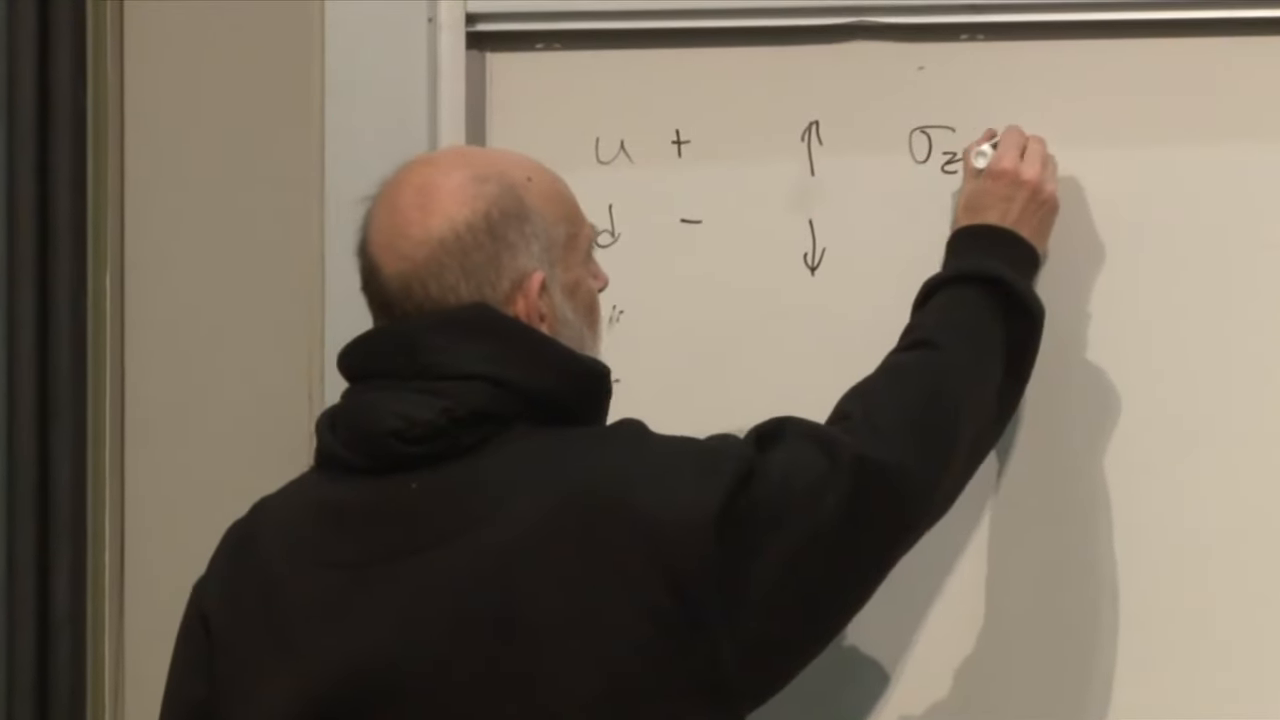
\includegraphics[width=0.78\textwidth]{lecture_02_figure_05.png}
\caption{Die Tafel fasst Linearkombinationen und die konjugierte Vertauschung der Argumente im Skalarprodukt zusammen.}
\lectureframe{00:46:53}
\end{figure}

Das Quadrat der Länge eines Vektors ist
\begin{equation}
\|\ket{A}\|^2=\braket{A}{A}.
\end{equation}
Gleichung~\eqref{eq:conjugate-symmetry} zeigt, dass diese Zahl gleich ihrer eigenen komplex Konjugierten und somit reell ist; aus den Axiomen des Skalarprodukts folgt außerdem, dass sie nichtnegativ ist. Zwei Vektoren sind orthogonal, wenn
\begin{equation}
\braket{A}{B}=0.
\end{equation}
Die Dimension des Raums ist die größte Anzahl paarweise orthogonaler, von null verschiedener Richtungen, die sich wählen lassen.

\begin{classroomqa}
\audiencequestion{Muss jede Basis aus paarweise orthogonalen Vektoren bestehen?}
\lecturerresponse{Nein. Eine Basis muss lediglich linear unabhängig sein und den Raum aufspannen. Orthogonale Basen sind besonders praktisch, weil sich die Koeffizienten und Wahrscheinlichkeiten leicht bestimmen lassen. In zwei Dimensionen können zwei nicht parallele Vektoren eine Basis bilden, auch wenn ihr Skalarprodukt nicht null ist.}
\end{classroomqa}

\section{Der zweidimensionale Spinraum}

Für den Zustandsraum eines einzelnen Spins postulieren wir einen zweidimensionalen komplexen Vektorraum,
\begin{equation}
\mathcal H_{\mathrm{spin}}\cong\mathbb C^2.
\end{equation}
Es gibt kontinuierlich viele mögliche Zustandsvektoren, doch zur Darstellung jedes beliebigen Zustands genügen zwei linear unabhängige Basisvektoren.

Beginnen wir mit den Zuständen, die ein entlang \(z\) ausgerichteter Apparat präpariert:
\begin{align}
\ket{u}&\longleftrightarrow \sigma_z=+1,\\
\ket{d}&\longleftrightarrow \sigma_z=-1.
\end{align}
Die Buchstaben \(u,d\), die Vorzeichen \(+,-\) und die Pfeile \(\uparrow,\downarrow\) sind alternative Bezeichnungen für dieselben beiden Präparationen. Da eine \(z\)-Messung sie mit Sicherheit unterscheidet, sind ihre Zustandsvektoren orthogonal:
\begin{equation}
\braket{u}{d}=0.
\end{equation}
Wir wählen ihre Länge gleich eins,
\[
\braket{u}{u}=\braket{d}{d}=1.
\]

Dann lässt sich jeder Spin-Zustand schreiben als
\begin{equation}
\ket{A}=\alpha_u\ket{u}+\alpha_d\ket{d},
\qquad \alpha_u,\alpha_d\in\mathbb C.
\label{eq:general-spin-state}
\end{equation}
Die Wahrscheinlichkeitsregel lautet
\begin{equation}
P(u|A)=|\alpha_u|^2,\qquad
P(d|A)=|\alpha_d|^2.
\label{eq:born-z}
\end{equation}
Da eines der beiden Ergebnisse eintreten muss, gilt
\begin{equation}
|\alpha_u|^2+|\alpha_d|^2=1.
\label{eq:normalization}
\end{equation}

\begin{figure}[htbp]
\centering
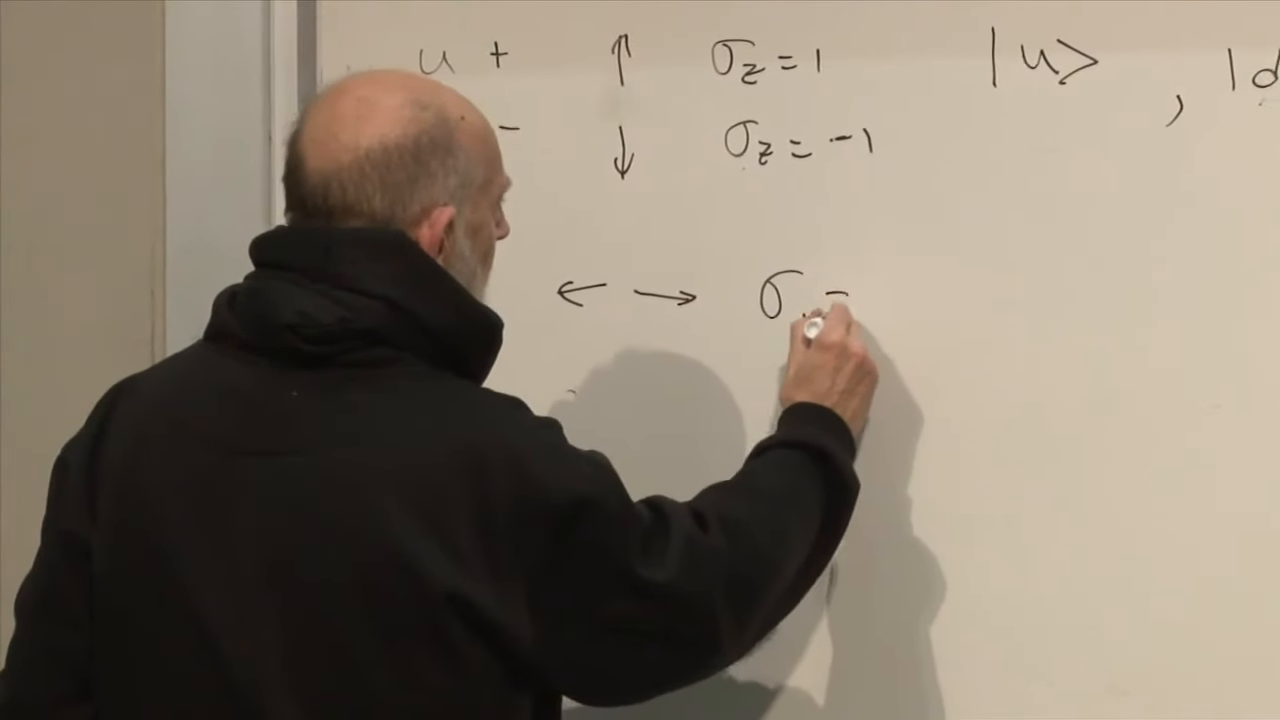
\includegraphics[width=0.78\textwidth]{lecture_02_figure_06.png}
\caption{Eine allgemeine Entwicklung in up--down, die Summe der Wahrscheinlichkeiten beider Ergebnisse und die äquivalente Bedingung der Einheitsnorm.}
\lectureframe{01:03:38}
\end{figure}

Die Äquivalenz mit der Normierung auf eins folgt unmittelbar:
\begin{align}
\braket{A}{A}
&=(\alpha_u^*\bra{u}+\alpha_d^*\bra{d})
  (\alpha_u\ket{u}+\alpha_d\ket{d})\\
&=|\alpha_u|^2\braket{u}{u}
 +\alpha_u^*\alpha_d\braket{u}{d}\\
&\quad +\alpha_d^*\alpha_u\braket{d}{u}
 +|\alpha_d|^2\braket{d}{d}\\
&=|\alpha_u|^2+|\alpha_d|^2=1.
\end{align}
Ein physikalischer reiner Zustand wird somit durch einen normierten Vektor dargestellt.

\begin{classroomqa}
\audiencequestion{Werden diese Aussagen hergeleitet, oder sind es Postulate?}
\lecturerresponse{An diesem Punkt sind dies die Regeln, die an die Experimente angepasst werden. Der zweidimensionale Raum, die Wahrscheinlichkeitsregel und die Deutung der Orthogonalität werden heuristisch eingeführt. Ihre gegenseitige Konsistenz lässt sich bereits jetzt überprüfen; als Nächstes folgt der systematische Zusammenhang zwischen Zuständen und Observablen.}
\end{classroomqa}

\subsection{Orthogonalität als Unterscheidbarkeit}

Der physikalische Gehalt der Orthogonalität ist hilfreicher als das Bild senkrechter Pfeile:

\begin{quote}Zustände, die sich durch eine Messung mit Sicherheit unterscheiden lassen, werden durch orthogonale Vektoren dargestellt.
\end{quote}

Up und down erfüllen dieses Kriterium. Ist der Zustand up, zeigt der \(z\)-Apparat niemals down, und umgekehrt. Ein von null verschiedenes Skalarprodukt bedeutet, dass ein Zustand gelegentlich ein Ergebnis hervorbringen kann, das mit dem anderen Zustand verknüpft ist.

\section{Die right--left-Basis}

Seien \(\ket{r}\) und \(\ket{l}\) die Zustände mit eindeutigem \(x\)-Spin:
\[
\ket{r}\longleftrightarrow\sigma_x=+1,\qquad
\ket{l}\longleftrightarrow\sigma_x=-1.
\]
Da der Raum zweidimensional ist, muss sich jeder dieser Zustände als Linearkombination von \(\ket{u}\) und \(\ket{d}\) schreiben lassen. Ein als right präparierter Spin ergibt up und down mit gleicher Wahrscheinlichkeit; daher müssen die beiden Koeffizienten denselben Betrag haben. Wir wählen die einfachste Phasenkonvention:
\begin{equation}
\ket{r}=\frac{1}{\sqrt2}\bigl(\ket{u}+\ket{d}\bigr).
\label{eq:right-state}
\end{equation}
Der Messapparat entlang \(x\) unterscheidet right und left mit Sicherheit, daher muss der Zustand left orthogonal zum Zustand right sein. Eine passende Wahl ist
\begin{equation}
\ket{l}=\frac{1}{\sqrt2}\bigl(\ket{u}-\ket{d}\bigr).
\label{eq:left-state}
\end{equation}
Tatsächlich gilt
\begin{align}
\braket{l}{r}
&=\frac12(\bra{u}-\bra{d})(\ket{u}+\ket{d})\\
&=\frac12(1-1)=0.
\end{align}

\begin{figure}[htbp]
\centering
\includegraphics[width=0.82\textwidth]{lecture_02_figure_07.png}
\caption{Die vollständige Konstruktion von right--left: gleiche Beträge der Koeffizienten für up--down, entgegengesetzte relative Vorzeichen und verschwindendes Skalarprodukt.}
\lectureframe{01:12:15}
\end{figure}

Das globale Minuszeichen von \(\ket{l}\) ist Konvention. Ersetzt man \(\ket{l}\) durch \(-\ket{l}\), ändern sich keine Wahrscheinlichkeiten. Addiert man Gleichung~\eqref{eq:right-state} und Gleichung~\eqref{eq:left-state} und zieht sie voneinander ab, erhält man die inverse Basisänderung:
\begin{align}
\ket{u}&=\frac{1}{\sqrt2}\bigl(\ket{r}+\ket{l}\bigr),\\
\ket{d}&=\frac{1}{\sqrt2}\bigl(\ket{r}-\ket{l}\bigr).
\end{align}
Diese Symmetrie ist wichtig. Ausgehend von der \(x\)-Basis ist up oder down eine Superposition mit gleichen Gewichten aus right und left – ebenso wie right oder left eine Superposition mit gleichen Gewichten aus up und down ist.

\section{Die in--out-Basis und die relative Phase}

Richten wir den Apparat entlang \(y\), also senkrecht zur Tafel, aus. Wir schreiben
\[
\ket{i}\longleftrightarrow\sigma_y=+1,\qquad
\ket{o}\longleftrightarrow\sigma_y=-1,
\]
Dabei bedeutet das Ket-Label \(i\) \emph{in}, während das unverzierte \(i\), das vor einem Ket steht, weiterhin die imaginäre Einheit bezeichnet.

Gleiche Wahrscheinlichkeiten für up und down erfordern Koeffizienten mit gleichem Betrag. Damit in und out orthogonal sind, muss eine relative Phase ihr Skalarprodukt verschwinden lassen. Eine symmetrische Wahl ist
\begin{align}
\ket{i}&=\frac{1}{\sqrt2}\bigl(\ket{u}+i\ket{d}\bigr),\\
\ket{o}&=\frac{1}{\sqrt2}\bigl(\ket{u}-i\ket{d}\bigr).
\label{eq:in-out-states}
\end{align}
In der Basis \((u,d)\) lauten alle sechs Zustände
\begin{align}
\ket{u}&=\binom10,
&
\ket{d}&=\binom01,
\\
\ket{r}&=\frac1{\sqrt2}\binom11,
&
\ket{l}&=\frac1{\sqrt2}\binom1{-1},
\\
\ket{i}&=\frac1{\sqrt2}\binom1{i},
&
\ket{o}&=\frac1{\sqrt2}\binom1{-i}.
\end{align}

\begin{figure}[htbp]
\centering
\includegraphics[width=0.82\textwidth]{lecture_02_figure_08.png}
\caption{Die sechs Spaltenvektoren in der up--down-Basis. Das untere Paar unterscheidet sich durch das Vorzeichen der relativen imaginären Phase.}
\lectureframe{01:20:50}
\end{figure}

Die komplexe Konjugation im Bra ist für die Überprüfung der Orthogonalität entscheidend:
\begin{align}
\braket{i}{o}
&=\frac12(\bra{u}-i\bra{d})(\ket{u}-i\ket{d})\\
&=\frac12\bigl(1+(-i)(-i)\bigr)=0.
\end{align}

\begin{classroomqa}
\audiencequestion{Drückt die Wahl von \(+i\) für \emph{ein} statt für \emph{aus} die Händigkeit der räumlichen Achsen aus?}
\lecturerresponse{Hier kommt eine Konvention ins Spiel, deren geometrische Bedeutung klarer wird, wenn die Pauli-Matrizen und Drehungen eingeführt werden. Für den Moment muss das Paar orthogonal und symmetrisch zu den anderen Basen angeordnet sein; eine Vertauschung der Bezeichnungen oder eine Umkehrung der \(y\)-Achse ändert die Konvention, nicht aber die Konsistenz der Konstruktion.}
\end{classroomqa}

\subsection{Überprüfung der Symmetrie in der right--left-Basis}

Verwenden wir
\[
\ket{u}=\frac{\ket{r}+\ket{l}}{\sqrt2},\qquad
\ket{d}=\frac{\ket{r}-\ket{l}}{\sqrt2}
\]für den Zustand in:
\begin{align}
\ket{i}
&=\frac1{\sqrt2}
\left(
\frac{\ket{r}+\ket{l}}{\sqrt2}
+i\frac{\ket{r}-\ket{l}}{\sqrt2}
\right)\\
&=\frac{1+i}{2}\ket{r}
 +\frac{1-i}{2}\ket{l}.
\label{eq:in-in-rl}
\end{align}
Obwohl keiner der beiden Koeffizienten sichtbar \(1/\sqrt2\) enthält, gilt
\begin{equation}
\left|\frac{1+i}{2}\right|^2
=\left|\frac{1-i}{2}\right|^2
=\frac12.
\end{equation}

\begin{figure}[htbp]
\centering
\includegraphics[width=0.82\textwidth]{lecture_02_figure_09.png}
\caption{Die vollständige Basisänderung für den Zustand in und die Überprüfung, dass die Wahrscheinlichkeiten für right--left jeweils \(1/2\) betragen.}
\lectureframe{01:29:10}
\end{figure}

Somit ergeben sich für jeden Zustand aus einer der drei Basen bei einer Messung in einer der beiden anderen Basen gleiche Wahrscheinlichkeiten. Die Basen \(z\), \(x\) und \(y\) sind paarweise zueinander unverzerrt.

\section{Warum es drei ausgezeichnete Basenpaare gibt}

\begin{classroomqa}
\audiencequestion{Kann es ein viertes Paar von Zuständen geben, das zu diesen drei Paaren genauso symmetrisch steht wie diese zueinander?}
\lecturerresponse{Nicht für ein einzelnes Zweizustandssystem. Sobald die drei zueinander unverzerrten Paare festgelegt sind, gibt es kein viertes Paar mit derselben Beziehung gleicher Überlappungen. Dass es drei solche räumlichen Bezeichnungen gibt, hängt mit den drei Dimensionen des gewöhnlichen Raums zusammen, obwohl der komplexe Zustandsraum selbst zweidimensional ist.}
\end{classroomqa}

Dieser Zusammenhang lässt sich durch Zählen der physikalischen Parameter erkennen. Eine allgemeine Spalte
\[
\binom{\alpha_u}{\alpha_d}
\]
enthält zwei komplexe Zahlen, also vier reelle Zahlen. Die Normierung liefert eine Bedingung:
\[
|\alpha_u|^2+|\alpha_d|^2=1.
\]
Eine Multiplikation beider Einträge mit derselben Phase ändert keine Messwahrscheinlichkeit:
\begin{equation}
\ket{A}\sim e^{i\chi}\ket{A}.
\label{eq:global-phase}
\end{equation}
Damit entfällt ein weiterer reeller Parameter. Es bleiben also
\begin{equation}
4-1-1=2
\end{equation}
physikalische reelle Parameter – genau so viele Winkel, wie zur Angabe einer Richtung im dreidimensionalen Raum nötig sind.

Eine praktische Repräsentation macht den Zusammenhang explizit:
\begin{equation}
\ket{\psi(\theta,\phi)}
=\cos\frac{\theta}{2}\,\ket{u}
+e^{i\phi}\sin\frac{\theta}{2}\,\ket{d}.
\label{eq:bloch-parameterization}
\end{equation}
\editorialnote{Gleichung~\eqref{eq:bloch-parameterization} ist die übliche normierte Repräsentation der von der Vorlesung identifizierten zweiparametrigen Familie. Die explizite Form mit halben Winkeln veranschaulicht die Parameterzählung; ihre dynamische und rotatorische Deutung gehört in spätere Vorlesungen.}

\begin{classroomqa}
\audiencequestion{Was bedeutet es mathematisch genau, die globale Phase zu ignorieren?}
\lecturerresponse{Alle normierten Vektoren auf dem Kreis \(\{e^{i\chi}\ket{\psi}\}\) stellen denselben physikalischen Zustand dar. Man erklärt diese Vektoren für äquivalent, ähnlich wie Punkte, die durch eine festgelegte Redundanz miteinander verbunden sind, als ein einziger physikalischer Punkt behandelt werden. Die relative Phase zwischen Komponenten bleibt messbar; nur eine Phase, mit der der gesamte Vektor multipliziert wird, bleibt unberücksichtigt.}
\end{classroomqa}

\begin{classroomqa}
\audiencequestion{Können in einer Rechnung auch nicht normierte Vektoren oder Vektoren mit negativen Komponenten vorkommen?}
\lecturerresponse{Ja. Die lineare Algebra lässt sie zu, und ein Zwischenvektor muss noch keinen präparierten physikalischen Zustand darstellen. Ein von null verschiedener Vektor kann am Ende normiert werden. Negative und komplexe Komponenten sind Amplituden, keine negativen Wahrscheinlichkeiten; Wahrscheinlichkeiten ergeben sich aus den Betragsquadraten, nachdem der Zustand normiert wurde.}
\end{classroomqa}

\begin{classroomqa}
\audiencequestion{Was geschieht mit diesem Bild in höherdimensionalen Räumen oder bei komplizierteren Spinoren?}
\lecturerresponse{Dieselben linearen Prinzipien gelten weiterhin, doch der Zusammenhang zwischen der Dimension des Zustandsraums, räumlichen Drehungen und beobachtbarem Spin wird reichhaltiger. Diese Erweiterung liegt außerhalb der vorliegenden Zweizustandskonstruktion.}
\end{classroomqa}

\section{Orthogonalität ist nicht räumliche Senkrechtstellung}

Das Wort \emph{orthogonal} hat nun eine abstrakte, operationelle Bedeutung. Es darf nicht mit dem Winkel zwischen zwei Pfeilen im gewöhnlichen Raum verwechselt werden. Die räumlichen Richtungen up und down sind entgegengesetzt, doch die Zustandsvektoren \(\ket{u}\) und \(\ket{d}\) sind orthogonal. Die räumlichen Richtungen up und right stehen senkrecht aufeinander, doch
\begin{equation}
\braket{u}{r}=\frac1{\sqrt2}\ne0.
\end{equation}

\begin{classroomqa}
\audiencequestion{Wie können entgegengesetzte räumliche Richtungen orthogonal sein, während zueinander senkrechte räumliche Richtungen es nicht sind?}
\lecturerresponse{Die Überlappung im Zustandsraum beschreibt die experimentelle Unterscheidbarkeit, nicht den euklidischen Winkel zwischen den Bezeichnungen. Up und Down lassen sich mit einer einzigen \(z\)-Messung mit Sicherheit unterscheiden, daher ist ihre Überlappung null. Up und Right lassen sich nicht mit Sicherheit unterscheiden: Bei einem in Right präparierten Spin tritt manchmal das Ergebnis Up auf. Daher überlappen sich ihre Zustandsvektoren.}
\end{classroomqa}

Dieselbe Idee hat ein klassisches probabilistisches Gegenstück. Zwei Wahrscheinlichkeitsverteilungen mit disjunktem Träger sind perfekt unterscheidbar: Ein beobachtetes Ergebnis zeigt, welche Verteilung vorlag. Verteilungen mit überlappendem Träger lassen sich anhand einer einzigen Stichprobe nicht fehlerfrei unterscheiden. Quantenmechanische Orthogonalität entspricht dem Fehlen einer Überlappung; ein von null verschiedenes Skalarprodukt zeigt an, dass manche Ergebnisse mit beiden Präparationen vereinbar sind.

\begin{classroomqa}
\audiencequestion{Sollte man sich den zweidimensionalen Zustandsraum als die physikalische Ebene vorstellen, in der die Pfeile Up und Right liegen?}
\lecturerresponse{Nein. Die Bezeichnungen \(x,y,z\) beziehen sich auf Orientierungen der Apparatur im gewöhnlichen Raum. Die Kets gehören zu einem komplexen Vektorraum mit einem eigenen Skalarprodukt. Die Anzahl der Parameter verknüpft die beiden Strukturen, doch sie Punkt für Punkt mit denselben Bildern gleichzusetzen, würde räumliche Senkrechtstellung mit Orthogonalität im Zustandsraum verwechseln.}
\end{classroomqa}

\section{Zustände, Messungen und die noch offenen Fragen}

Die Konstruktion ist bislang dadurch vorangeschritten, dass Vektoren an operationelle Fakten angepasst wurden. Die drei Ausrichtungen des Apparats kennzeichnen drei Paare normierter Zustände, und die Überlappungen geben die beobachteten Wahrscheinlichkeiten wieder. Eine rigorose Behandlung muss noch angeben, wie eine Observable wie \(\sigma_z\) auf einen Zustand wirkt und warum ihre möglichen Messergebnisse ihre Eigenwerte sind. Das ist der nächste Schritt.

Das frühere logische Rätsel lässt sich nun präziser formulieren. Aussagen entsprechen Unterräumen oder ihren Projektoren, und nicht kompatible Projektoren kommutieren nicht. Der reihenfolgeabhängige ODER-Test war kein sprachliches Paradoxon, sondern ein frühes Auftreten dieser nichtkommutativen Struktur.

\begin{classroomqa}
\audiencequestion{Wenn der Zustand kein gewöhnlicher Pfeil ist, warum wirken die drei Bezeichnungen \(x,y,z\) und der Mittelwert \(\langle\sigma_{\hat m}\rangle\) dann so klassisch?}
\lecturerresponse{Der klassische Vektor tritt in Ensemblemittelwerten auf. Ein einzelner Spin liefert ein diskretes Ergebnis, während viele identisch präparierte Spins Mittelwerte ergeben, die sich wie die Komponenten einer Richtung transformieren. Klassisches makroskopisches Verhalten entsteht, wenn große Ansammlungen diese Mittelwerte stabil machen; daraus sollte man nicht rückwärts auf einen verborgenen kontinuierlichen Wert für jeden einzelnen Spin schließen.}
\end{classroomqa}

\begin{classroomqa}
\audiencequestion{Ist die Redundanz der gemeinsamen Phase ein Beispiel für Eichinvarianz?}
\lecturerresponse{Es handelt sich um eine einfache Invarianz gegenüber einer gemeinsamen Phase, die umfassendere Eichideen vorwegnimmt. Eine Ausarbeitung dieses Zusammenhangs würde hier über den Rahmen der vorliegenden Konstruktion hinausgehen. Daher wird nur die physikalisch relevante Aussage festgehalten: Eine gemeinsame Phase ist unbeobachtbar, eine relative Phase dagegen nicht.}
\end{classroomqa}

Schließlich sollte man sich eine Messung nicht so vorstellen, als decke sie lediglich einen Wert auf, den der Spin schon immer im klassischen Sinn besessen hätte. Sie präpariert den Zustand, der dem aufgezeichneten Ergebnis entspricht. Eine unmittelbar anschließende Wiederholung derselben Messung ist daher damit vereinbar, während ein neues Ensemble identisch präparierter Spins die durch die entsprechenden Amplituden bestimmte Wahrscheinlichkeitsverteilung zeigt. Die mathematische Beschreibung dieser Präparation und Auslesung wird präzise, sobald Observable als Operatoren eingeführt werden.